\documentclass[12pt,a4paper]{report}
\usepackage[utf8]{vietnam}
\usepackage{amsmath}
\usepackage{amssymb}
\usepackage{graphicx}
\usepackage[left=2cm,right=2cm,top=2cm,bottom=2cm]{geometry}
\usepackage[unicode]{hyperref}
\usepackage{indentfirst}
\usepackage{lmodern}
\usepackage{listings}
\usepackage{color}
\usepackage{titlesec}

\titleformat*{\section}{\LARGE\bfseries}
\titleformat*{\subsection}{\Large\bfseries}
\titleformat*{\subsubsection}{\large\bfseries}

\definecolor{dkgreen}{rgb}{0,0.6,0}
\definecolor{gray}{rgb}{0.5,0.5,0.5}
\definecolor{mauve}{rgb}{0.58,0,0.82}

\lstset{frame=tb,
  language=C++,
  aboveskip=3mm,
  belowskip=3mm,
  showstringspaces=false,
  columns=flexible,
  basicstyle={\large\ttfamily},
  numbers=none,
  numberstyle=\tiny\color{gray},
  keywordstyle=\color{blue},
  commentstyle=\color{dkgreen},
  stringstyle=\color{mauve},
  breaklines=true,
  breakatwhitespace=true,
  tabsize=3
}
\begin{document}
    \begin{center}
    \LARGE\textbf{TRƯỜNG ĐẠI HỌC CÔNG NGHỆ THÔNG TIN}\\
    \LargeĐẠI HỌC QUỐC GIA TP HCM \\

    \LARGE\textbf{KHOA KHOA HỌC MÁY TÍNH}
        \begin{figure}[ht]
            \begin{center}
                
\includegraphics[scale=1.0]{logo.jpg}\\
            \end{center}
        \end{figure}
    \LARGE\textbf{BÁO CÁO ĐỒ ÁN }

    \LARGE\textbf{PHÂN TÍCH VÀ THIẾT KẾ THUẬT TOÁN}
    
    \LARGE\textbf {KNAPSACK}

    Lớp: CS112.L11

    GVHD: Phạm Nguyễn Trường An

    Sinh viên thực hiện:

    16521692 - Nguyễn Vĩnh Huy
    \end{center}
    \begin{figure}[ht]
        \begin{center}
        
\includegraphics[scale=1.0]{a.jpg}\\
        \end{center}
        \end{figure}
    \tableofcontents
    \chapter{0-1 Knapsack}
    \section{Giới thiệu bài toán}
    Bài toán Knapsack, hay còn gọi là xếp ba lô, hay bài toán cái túi,
    là một bài toán \textit{Tối ưu hóa tổ hợp}. Bài toán được đặt tên từ vấn đề
    chọn những gì quan trọng để có thể chứa vừa vào một cái túi (với giới hạn khối
    lượng) để mang theo trong một chuyến đi. Ở đây, ta cho rằng các đồ vật
    không thể bị chia nhỏ/xé nhỏ/tách nhỏ ra.

    Các bài toán tương tự thường xuất hiện trong kinh doanh, toán tổ hợp, lý thuyết
    độ phức tạp tính toán và mật mã học.
    
    \section{Liên hệ thực tế}
    Với việc một sinh viên mới lên thành phố, thường hay về nhà vào mỗi cuối tuần, 
    thì có thể áp dụng Knapsack vào để giải quyết các đồ vật vào ba lô để tổng giá 
    trị của đồ vật mang về nhà là nhiều nhất. 
    \section{Phát biểu bài toán}
    Cho một cái túi có thể chứa một khối lượng W, hai mảng số nguyên là 
    val[0..n-1] và wt[0..n-1] lần lượt là giá trị và trọng lượng của đồ vật n.
    Tìm một tập hợp các đồ vật sao cho nhét vừa vào ba lô và tổng giá trị của
    các đồ vật mang đi là lớn nhất.
    
    \textbf{Input}:
    \begin{itemize}
        \item W: Sức chứa của túi
        \item mảng val: giá trị của n đồ vật
        \item mảng wt: trọng lượng của n đồ vật
    \end{itemize}
    \textbf{Output}:
    \begin{itemize}
        \item max: Tổng giá trị tối đa mà túi mang đi được
    \end{itemize}

    Bài toán Knapsack là một trong những bài toán có độ phức tạp là Pseudo polynomial
    (tạm dịch: Giả đa thức). 

    \section{Độ phức tạp Pseudo Polynomial}
    Độ phức tạp Pseudo polynomial là độ phức tạp mà thời
    gian chạy trong trường hợp xấu nhất (worst case time complexity) 
    bị phụ thuộc vào giá trị số học(numeric value) của Input thay vì số 
    lượng input (number of inputs).

    Ví dụ: Xét bài toán đếm số lần xuất hiện của tất cả các phần tử trong một
    mảng số nguyên dương. Ta có thể cài đặt một phương pháp giả đa thức cho 
    bài toán này. Trước tiên tìm giá trị lớn nhất trong mảng, sau đó lặp từ giá 
    trị 1 đến giá trị lớn nhất này và đối với mỗi giá trị, tìm số lần xuất hiện
    của nó trong mảng. 

    \chapter{Phương pháp thiết kế bài toán}
    \section{Đệ quy}
    \subsection{Giới thiệu phương pháp}
    \textit{Đệ quy} xảy ra khi bên trong một khái niệm X có sử dụng chính khái 
    niệm X. Trong lập trình, \textit{Đệ quy} xảy ra khi một phương thức được viết
    tự gọi lại chính nó.
    Ví dụ: Mã giả của hàm tính Fibbonacci
    \begin{lstlisting}
    Fibo(n)
    if n <= 1 then
       return 1
    else
       return Fibo(n-1) + Fibo(n-2)
    \end{lstlisting}
    Hai yếu tố cần để tạo thành một phương thức đệ quy:
    \begin{itemize}
        \item Điều kiện dừng: Xác định cụ thể quy luật của phương thức và tìm giá 
    trị cụ thể cho đến khi thỏa mãn một điều kiện nhất định.
        \item Phương thức đệ quy: Phương thức đệ quy sẽ tự gọi lại chính nó cho đến khi
    nó trả về điều kiện dừng.
    \end{itemize}

    \subsection{Mã giả}
    \begin{lstlisting}
        knapSack(W, wt, val, n): 
            if n = 0 or W = 0  
                return 0
            if wt[n-1] > W
                return knapSack(W, wt, val, n-1) 
            else: 
                return max( 
                    val[n-1] + knapSack( 
                        W-wt[n-1], wt, val, n-1), 
                    knapSack(W, wt, val, n-1)) 
    \end{lstlisting}
    \subsection{Phân tích độ phức tạp bằng các phương pháp toán học}
    Ta có phương trình đệ quy:
    \begin{align}
        \begin{cases}
            T(0) = 1 \\
            T(n) = O(1) + 2T(n-1), n>0 
        \end{cases}
    \end{align}
    Giải hệ phương trình này, ta được:\\
    \begin{math}
        T(n) = 3O(1) + 4T(n-2) \\
        T(n) = 7O(1) + 8T(n-3) \\ 
        ... \\
        T(n) = (2^{n-1} - 1)O(1) + 2^{n-1}T(1)\\
        T(n) = (2^n-1)O(1)\\
        T(n) = O(2^n)
    \end{math}
    
    
    Với phương pháp giải quyết bài toán bằng đệ quy, ta không tốn chi phí phụ 
    thêm cho việc lưu trữ các biến tạm, nên độ phức tạp về mặt không gian lưu trữ 
    (Space Complexity) là O(1)
    \subsection{Mã nguồn}
    knapsackR.py
    \begin{lstlisting}
        class knapsackRecursion:
            complexity = 0
            wt = []
            val = []
            W = 0
            n = 0
            ketqua = 0
            def __init__ (self, W, n, wt, val):
                self.W = W
                self. wt = wt
                self. n = n
                self.val = val 
            def knapSack(self, W, n, wt, val):
                self.complexity += 2 
                if n == 0 or W == 0:
                    return 0
                self.complexity += 1    
                if (wt[n-1] > W):  
                    return self.knapSack(W, n - 1, wt, val) 
                else: 
                    return max( 
                        val[n-1] + self.knapSack( 
                            W-wt[n-1], n - 1, wt, val), 
                        self.knapSack(W, n - 1, wt, val)) 
            
            def Solve(self):
                self.ketqua = self.knapSack(self.W, self.n, self.wt, self.val)
            
    
    \end{lstlisting}
    \subsection{Phát sinh intput/output để kiểm tra tính đúng đắn}
    Input của bài toán được phát sinh ngẫu nhiên bằng cách sử dụng hàm randrange có
    sẵn trong python. Input được phát sinh ngẫu nhiên, sau đó tính Output bằng 
    thư viện OR-tools . Mã nguồn phát sinh Input/Output:
    generator.py
    \begin{lstlisting}
        import random
        from ortools.algorithms import pywrapknapsack_solver   
        def generator(W, n, filename = None, output = None):
            wt = []
            val = []
            for i in range (n):
                wt.append(random.randrange(100))
                val.append(random.randrange(100))
        
            solver = pywrapknapsack_solver.KnapsackSolver(
                pywrapknapsack_solver.KnapsackSolver.
                KNAPSACK_MULTIDIMENSION_BRANCH_AND_BOUND_SOLVER, 'KnapsackExample')
        
            solver.Init(val, [wt], [W])
            bestvalue = solver.Solve()
            if filename:
                file = open(filename,"w")
                file.write(str(n) + " " + str(W) + " " + str(bestvalue) + "\n")
                for i in range (n):
                    file.write(str(wt[i]) + " " + str(val[i])+ "\n")
            if output != None:
                print("W = ",W)
                print("n = ", n)
                print("wt = ", wt)
                print("val = ",val)
            return wt,val,bestvalue
    \end{lstlisting}
    Dùng hàm generator đã cài đặt trên để sinh ra ba file Test1.txt, Test2.txt,
    Test3.txt. Bên trong mỗi file có chứa dữ liệu với cấu trúc:
    \begin{itemize}
        \item Hàng 1: chứa n, W và kết quả tối ưu nhất
        \item n hàng tiếp theo: lần lượt chứa wt[0], val[0], wt[1], val[1]... 
        \item wt[n], val[n]: là cân nặng và giá trị của đồ vật
    \end{itemize}
    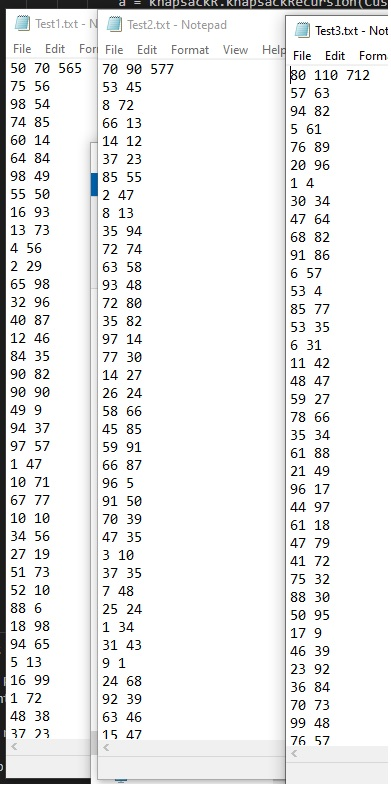
\includegraphics[scale=0.5]{test_showcase.jpg}

    (Nội dung chi tiết các file có đính kèm trong source code)
    Từ các file test đã tạo ở trên, ta có hàm test tính đúng đắn của mã nguồn đã 
    cài đặt cho phương pháp trên. Ứng với mỗi file test, nếu phát hiện Output sai
    so với kết quả tính toán từ thư viện OR-tools, xuất ra "DP SAI VOI TEST i" (Với i
    là tên file test cho Output sai).

    Mã nguồn kiểm tra tính đúng đắn: 
    validate.py
    \begin{lstlisting}
        import inputReader
        import knapsackDP
        import knapsackR

        validDP = 1
        validR = 1
        for i in range(1,4):
            W, n, wt, val, result = inputReader.input_processing("Test"+str(i)+".txt")
            DP = knapsackDP.knapsackDP(W, n, wt, val)
            R = knapsackR.knapsackRecursion(W, n, wt, val)
            DP.Solve()
            R.Solve()
            if (DP.ketqua != result):
                validDP = 0
                print("DP SAI VOI TEST ", i)
            if (R.ketqua != result):
                validR = 0
                print("DE QUY SAI VOI TEST ",i)
        if (validDP):
            print("DP dung cho moi test")
        if (validR):
            print ("De quy dung cho moi test")
    \end{lstlisting}
    \subsection{Phân tích độ phức tạp bằng thực nghiệm}
    Với các file test đã sinh ra ở trên, ta tiếp tục sử dụng chúng trong việc phân
    tích độ phức tạp bằng thực nghiệm.

    Từ tính đúng đắn đã được kiểm chứng ở mục trên, mã nguồn cài đặt cho phương 
    pháp đệ quy đã được chứng minh là đúng. Từ các file test ở trên, bỏ qua việc sử 
    dụng tải trọng W có bên trong file, ta sử dụng một "CustomW". CustomW này 
    có giá trị trong khoảng (W,W+50), và mỗi CustomW sẽ cách nhau một khoảng bằng 10. 

    Ứng với mỗi file test, ta sử dụng lại toàn bộ các giá trị của mảng val, mảng wt,
    n, tuy nhiên, W sẽ được thay thế bằng CustomW như đã nói trên, và result sẽ được
    tính lại ứng với mỗi W = CustomW.

    Độ phức tạp của thuật toán được tính bằng tổng số phép toán trong quá trình chạy.
    Tổng số phép toán trong quá trình chạy là tổng của số phép gán và số phép so sánh.
    Với mỗi phép so sánh, tổng số phép toán tăng lên 1. Tương tự, với mỗi phép so sánh
    tổng số phép toán cũng tăng lên 1. Và với mỗi lần duyệt mảng, ta tính nó tương tự 
    như thực hiện một lần phép so sánh.

    Ứng với mỗi CustomW, ngoài việc thực hiện đo số phép toán, ta còn đo cả thời gian 
    giải bài toán (Tính theo giây) và sau đó xuất ra màn hình.


    Mã nguồn thực hiện việc kiểm tra độ phức tạp:


    analysisR.py
    \begin{lstlisting}
        import knapsackR
        import inputReader
        import time

        for i in range (1,4):
            W, n, wt, val, result = inputReader.input_processing("Test"+str(i)+".txt")
            for CustomW in range (W, W + 50, 10):
                a = knapsackR.knapsackRecursion(CustomW, n, wt, val)
                start_time = time.time()
                a.Solve()
                print("Test case: ",i, "Custom W:", CustomW)
                print("Giai bai toan trong:",time.time() - start_time)
                print("Voi so phep toan: ", a.complexity)
    \end{lstlisting}

    Kết quả chạy thử:

    \begin{center}
        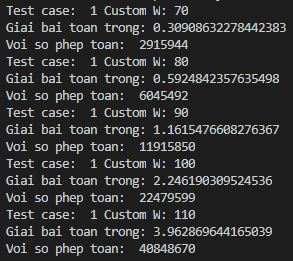
\includegraphics{RT1.JPG}
        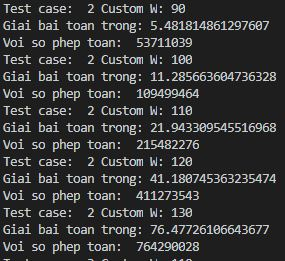
\includegraphics{RT2.JPG}
        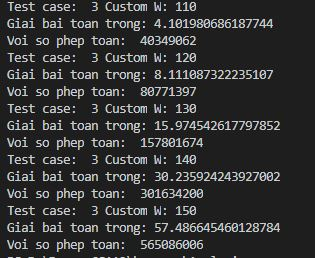
\includegraphics{RT3.JPG}
    \end{center}

    \section{Quy hoạch động}
    \subsection{Giới thiệu phương pháp}
    Quy hoạch động (Dynamic Programming) được phát triển bởi nhà toán học Richard Bellman từ thập niên 
    1950s. Thời đó Programming không có ý nghĩa là lập trình máy tính như hiện tại.
    Programming có nghĩa là "tính toán bằng cách lập bảng", hay còn gọi là quy hoạch.
    Quy hoạch động được dùng để giải các bài toán có dạng đệ quy.
    Các bước sử dụng Dynamic Programming:
    \begin{itemize}
        \item Tìm cách mô phỏng dạng thức "một lời giải" của bài toán.
        \item Tìm phương trình đệ quy để tính lời giải tối ưu.
        \item Sử dụng phương pháp đệ quy có nhớ (Top down with memoization) hoặc
    phương pháp tìm lời giải từ dưới lên bottom-up để code tính kết quả tối ưu.
    \end{itemize}
    \subsection{Mã giả}
    \begin{lstlisting}
    knapSack(W, wt, val, n)
        K = [][]
        for i = 0 to W + 1
            for j in range n + 1
                K[i][j] = 0
        for i = 0 to n + 1 
            for w = 0 to W + 1 
                if i == 0 or w == 0 
                    K[i][w] = 0
                elif wt[i-1] <= w
                    K[i][w] = max(val[i-1] 
                            + K[i-1][w-wt[i-1]],   
                                K[i-1][w]) 
                else
                    K[i][w] = K[i-1][w] 
        return K[n][W] 
    \end{lstlisting}
    \subsection{Phân tích độ phức tạp bằng các phương pháp toán học}
    Thuật toán gồm 2 vòng for chạy lồng vào nhau => 
    T(n) = O(n x W)
    Với phương pháp này, ta tốn thêm 1 bảng có độ lớn là n x W để lưu trữ các 
    biến tạm. Vậy nên, độ phức tạp về mặt không gian lưu trữ (Space Complexity) là
    O(n x W)
    \subsection{Mã nguồn}
    knapsackDP.py
    \begin{lstlisting}
        class knapsackDP:
            W = 0
            n = 0
            wt = []
            val = []
            sosanh = 0
            gan = 0
            duyetmang = 0
            ketqua = 0
            complexity = 0
            def __init__(self, W, n, wt, val):
                self.W = W
                self.n = n
                self. wt = wt
                self.val = val
        
            def knapSack(self, W, n, wt, val): 
                DEFAULTSPACEUSAGE = (W + 1) * (n + 1)
                self.sosanh += DEFAULTSPACEUSAGE
                self.gan += DEFAULTSPACEUSAGE
                K = [[0 for x in range(W + 1)] for x in range(n + 1)] 
                self.sosanh += DEFAULTSPACEUSAGE
                for i in range(n + 1):
                    for w in range(W + 1):
                        self.sosanh += 2 
                        if i == 0 or w == 0: 
                            K[i][w] = 0
                            self.gan += 1
                        elif wt[i-1] <= w: 
                            self.sosanh += 1
                            K[i][w] = max(val[i-1] 
                                    + K[i-1][w-wt[i-1]],   
                                        K[i-1][w])
                            self.gan += 1 
                        else: 
                            self.sosanh += 1
                            K[i][w] = K[i-1][w] 
                            self.gan += 1
                return K[n][W] 
            
            def Solve(self):
                self.ketqua = self.knapSack(self.W, self.n, self.wt, self.val)
                self.complexity = self.gan + self.sosanh
        
    \end{lstlisting}
    \subsection{Phát sinh intput/output để kiểm tra tính đúng đắn}
    Input của bài toán được phát sinh ngẫu nhiên bằng cách sử dụng hàm randrange có
    sẵn trong python. Input được phát sinh ngẫu nhiên, sau đó tính Output bằng 
    thư viện ortools.algorithms . Mã nguồn phát sinh Input/Output:

    generator.py
    \begin{lstlisting}
        import random
        from ortools.algorithms import pywrapknapsack_solver
        def generator(W, n, filename = None, output = None):
            wt = []
            val = []
            for i in range (n):
                wt.append(random.randrange(100))
                val.append(random.randrange(100))
        
            solver = pywrapknapsack_solver.KnapsackSolver(
                pywrapknapsack_solver.KnapsackSolver.
                KNAPSACK_MULTIDIMENSION_BRANCH_AND_BOUND_SOLVER, 'KnapsackExample')
        
            solver.Init(val, [wt], [W])
            bestvalue = solver.Solve()
            if filename:
                file = open(filename,"w")
                file.write(str(n) + " " + str(W) + " " + str(bestvalue) + "\n")
                for i in range (n):
                    file.write(str(wt[i]) + " " + str(val[i])+ "\n")
            if output != None:
                print("W = ",W)
                print("n = ", n)
                print("wt = ", wt)
                print("val = ",val)
            return wt,val,bestvalue
    \end{lstlisting}
    Dùng hàm generator đã cài đặt trên để sinh ra ba file Test1.txt, Test2.txt,
    Test3.txt. Bên trong mỗi file có chứa dữ liệu với cấu trúc:
    \begin{itemize}
        \item Hàng 1: chứa n, W và kết quả tối ưu nhất
        \item n hàng tiếp theo: lần lượt chứa wt[0], val[0], wt[1], val[1]... 
        \item wt[n], val[n]: là cân nặng và giá trị của đồ vật
    \end{itemize}
    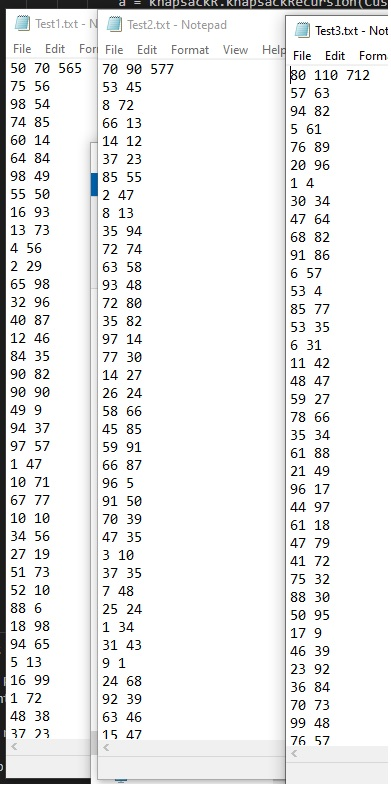
\includegraphics[scale=0.5]{test_showcase.jpg}

    (Nội dung chi tiết các file có đính kèm trong source code)
    Từ các file test đã tạo ở trên, ta có hàm test tính đúng đắn của mã nguồn đã 
    cài đặt cho phương pháp trên. Ứng với mỗi file test, nếu phát hiện Output sai
    so với kết quả tính toán từ thư viện OR-tools, xuất ra "DP SAI VOI TEST i" (Với i
    là tên file test cho Output sai).

    Mã nguồn kiểm tra tính đúng đắn: 
    validate.py
    \begin{lstlisting}
        import inputReader
        import knapsackDP
        import knapsackR

        validDP = 1
        validR = 1
        for i in range(1,4):
            W, n, wt, val, result = inputReader.input_processing("Test"+str(i)+".txt")
            DP = knapsackDP.knapsackDP(W, n, wt, val)
            R = knapsackR.knapsackRecursion(W, n, wt, val)
            DP.Solve()
            R.Solve()
            if (DP.ketqua != result):
                validDP = 0
                print("DP SAI VOI TEST ", i)
            if (R.ketqua != result):
                validR = 0
                print("DE QUY SAI VOI TEST ",i)
        if (validDP):
            print("DP dung cho moi test")
        if (validR):
            print ("De quy dung cho moi test")
    \end{lstlisting}
    \subsection{Phân tích độ phức tạp bằng thực nghiệm}
    Với các file test đã sinh ra ở trên, ta tiếp tục sử dụng chúng trong việc phân
    tích độ phức tạp bằng thực nghiệm.

    Từ tính đúng đắn đã được kiểm chứng ở mục trên, mã nguồn cài đặt cho phương 
    pháp đệ quy đã được chứng minh là đúng. Từ các file test ở trên, bỏ qua việc sử 
    dụng tải trọng W có bên trong file, ta sử dụng một "CustomW". CustomW này 
    có giá trị trong khoảng (W,W+50), và mỗi CustomW sẽ cách nhau một khoảng bằng 10. 

    Ứng với mỗi file test, ta sử dụng lại toàn bộ các giá trị của mảng val, mảng wt,
    n, tuy nhiên, W sẽ được thay thế bằng CustomW như đã nói trên, và result sẽ được
    tính lại ứng với mỗi W = CustomW.

    Độ phức tạp của thuật toán được tính bằng tổng số phép toán trong quá trình chạy.
    Tổng số phép toán trong quá trình chạy là tổng của số phép gán và số phép so sánh.
    Với mỗi phép so sánh, tổng số phép toán tăng lên 1. Tương tự, với mỗi phép so sánh
    tổng số phép toán cũng tăng lên 1. Và với mỗi lần duyệt mảng, ta tính nó tương tự 
    như thực hiện một lần phép so sánh.

    Ứng với mỗi CustomW, ngoài việc thực hiện đo số phép toán, ta còn đo cả thời gian 
    giải bài toán (Tính theo giây) và sau đó xuất ra màn hình.

    Mã nguồn thực hiện việc kiểm tra độ phức tạp cho cài đặt theo phương pháp
    Quy hoạch động: 

    analysisDP.py

    \begin{lstlisting}
        import knapsackDP
        import inputReader
        import time

        for i in range (1,4):
            W, n, wt, val, result = inputReader.input_processing("Test"+str(i)+".txt")
            for CustomW in range (W, W + 50, 10):
                a = knapsackDP.knapsackDP(CustomW, n, wt, val)
                start_time = time.time()
                a.Solve()
                print("Test case: ",i, "Custom W:", CustomW)
                print("Giai bai toan trong:",time.time() - start_time)
                print("Voi so phep toan: ", a.complexity)
    \end{lstlisting}

    Kết quả chạy thử:

    \begin{center}
        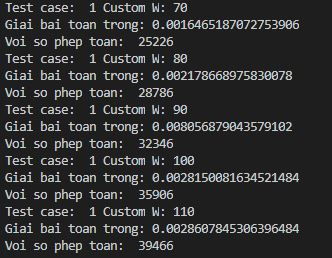
\includegraphics{DPT1.JPG}
        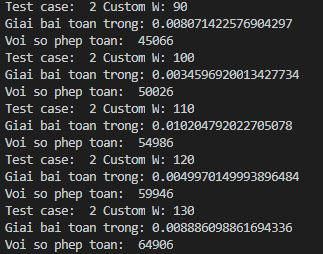
\includegraphics{DPT2.JPG}
        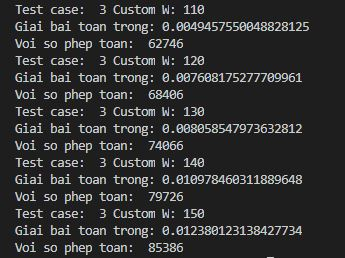
\includegraphics{DPT3.JPG}
    \end{center}

\end{document}
